\documentclass{beamer}

%% Juego de caracteres usado en el archivo fuente: UTF-8
\usepackage{ucs}
\usepackage[utf8x]{inputenc}
\uselanguage{spanish}
%Para la identación del español
\usepackage[spanish]{babel}

% There are many different themes available for Beamer. A comprehensive
% list with examples is given here:
% http://deic.uab.es/~iblanes/beamer_gallery/index_by_theme.html
% You can uncomment the themes below if you would like to use a different
% one:
%\usetheme{AnnArbor}
%\usetheme{Antibes}
%\usetheme{Bergen}
%\usetheme{Berkeley}
%\usetheme{Berlin}
%\usetheme{Boadilla}
%\usetheme{boxes}
%\usetheme{CambridgeUS}
%\usetheme{Copenhagen}
%\usetheme{Darmstadt}
%\usetheme{default}
%\usetheme{Frankfurt}
%\usetheme{Goettingen}
%\usetheme{Hannover}
%\usetheme{Ilmenau}
%\usetheme{JuanLesPins}
%\usetheme{Luebeck}
\usetheme{Madrid}
%\usetheme{Malmoe}
%\usetheme{Marburg}
%\usetheme{Montpellier}
%\usetheme{PaloAlto}
%\usetheme{Pittsburgh}
%\usetheme{Rochester}
%\usetheme{Singapore}
%\usetheme{Szeged}
%\usetheme{Warsaw}

%Para la identación del español
\usepackage[spanish]{babel}

\title{Apache Flink}

% A subtitle is optional and this may be deleted
%\subtitle{Optional Subtitle}

\author{Jesús Rodríguez Heras\\Roberto Muras González\\Juan Pedro Rodríguez Gracia\\Gabriel Fernando Sánchez Reina}
% - Give the names in the same order as the appear in the paper.
% - Use the \inst{?} command only if the authors have different
%   affiliation.

\institute[Escuela Superior de Ingeniería] % (optional, but mostly needed)
%{
%  \inst{1}%
%  Department of Computer Science\\
%  University of Somewhere
%  \and
%  \inst{2}%
%  Department of Theoretical Philosophy\\
%  University of Elsewhere}
% - Use the \inst command only if there are several affiliations.
% - Keep it simple, no one is interested in your street address.

%\date{March $8^{th}$, 2018}
% - Either use conference name or its abbreviation.
% - Not really informative to the audience, more for people (including
%   yourself) who are reading the slides online

%\subject{Theoretical Computer Science}
% This is only inserted into the PDF information catalog. Can be left
% out. 

% If you have a file called "university-logo-filename.xxx", where xxx
% is a graphic format that can be processed by latex or pdflatex,
% resp., then you can add a logo as follows:

% pgfdeclareimage[height=0.5cm]{university-logo}{university-logo-filename}
% \logo{\pgfuseimage{university-logo}}

% Delete this, if you do not want the table of contents to pop up at
% the beginning of each subsection:
%\AtBeginSubsection[]
%{
%  \begin{frame}<beamer>{Índice}
%    \tableofcontents[currentsection,currentsubsection]
%  \end{frame}
%}

% Let's get started
\begin{document}

\begin{frame}
  \titlepage
  
\end{frame}

\begin{frame}{Index}
  \tableofcontents
  % You might wish to add the option [pausesections]
\end{frame}

% Section and subsections will appear in the presentation overview
% and table of contents.


\section{Definiciones}
\subsection{Apache Flink}
\begin{frame}{¿Qué es Apache Flink?}
	\begin{block}{Apache Flink}
		Se trata de un motor de procesamiento de streams o flujos de datos de código abierto que proporciona capacidades de distribución de datos, comunicaciones y, muy importante, tolerancia a fallos a las computaciones.
	\end{block}
\end{frame}

\subsection{RabbitMQ}
\begin{frame}{¿Qué es Rabbit MQ?}
	\begin{block}{RabbitMQ}
		Es un software de negociación de mensajes de código abierto. Se encuentra dentro de la categoría de middleware de mensajería. Implementa el estándar ``Advanced Message Queuing Protocol'' (AMQP).
	\end{block}
\end{frame}

\section{Instalación}
\subsection{Java}
\begin{frame}{Java}
	\begin{block}{Instalación de java}
		Para la instalación de java, solo hay que descargarse el jdk de la página oficial e instalarlo en \texttt{/usr/java/}.
	\end{block}
\end{frame}

\subsection{Apache Flink}
\begin{frame}{Flink}
	\begin{block}{Instalación de Apache Flink}
		Para su instalación, nos descargamos el software desde su página web, lo descomprimimos donde queramos y ejecutamos el fichero \texttt{start-cluster.sh}.
	\end{block}
\end{frame}

\begin{frame}{Flink}
\begin{block}{Comprobamos que funciona}
	Para ello entramos en \texttt{localchost:8082}.
	\begin{center}
		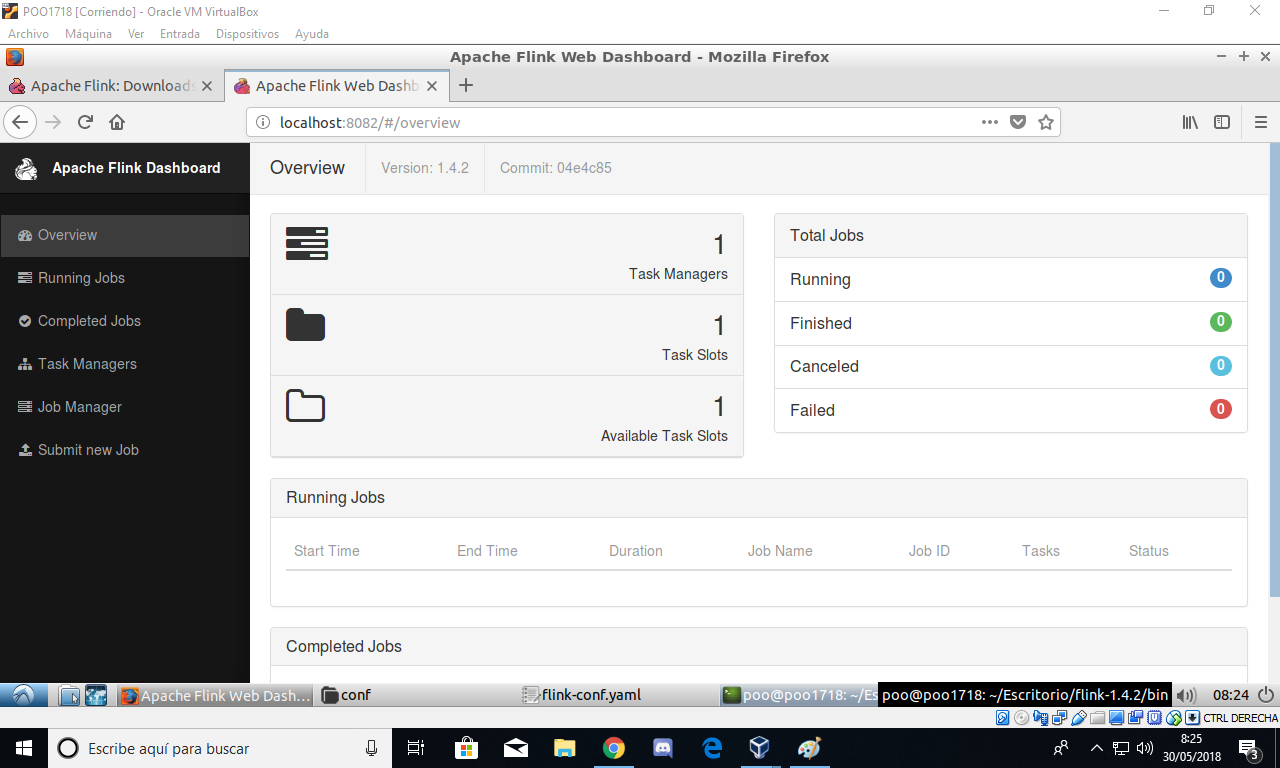
\includegraphics[scale=0.3]{9.png}
	\end{center}
\end{block}
\end{frame}

\subsection{RabbitMQ}
\begin{frame}{RabbitMQ}
	\begin{block}{Instalación de RabbitMQ}
		Para su instalación, introducimos el siguiente comando en la terminal:
		\begin{center}
			\texttt{sudo apte-get install rabbitmq-server}
		\end{center}
		Luego, instalamos la consola de administración con este comando:
		\begin{center}
			\texttt{sudo rabbitmq-plugins enable rabbitmq\_management}
		\end{center}
	\end{block}
\end{frame}

\section{Palabras más publicadas en twitter}
\begin{frame}{Palabras más publicadas en twitter}
\begin{block}{Funcionamiento}
	Nuestro trabajo consta de dos archivos Python:
	\begin{itemize}
		\item \texttt{tareas.py}.
		\item \texttt{receptor.py}.
		\item Ejecución del servicio de Apache Flink: \texttt{bin/flink run examples/batch/WordCount.jar -input /home/jesus/input.txt -output /home/jesus/output.txt}
	\end{itemize}
\end{block}	
\end{frame}

\begin{frame}{Palabras más publicadas en twitter}
	\begin{center}
		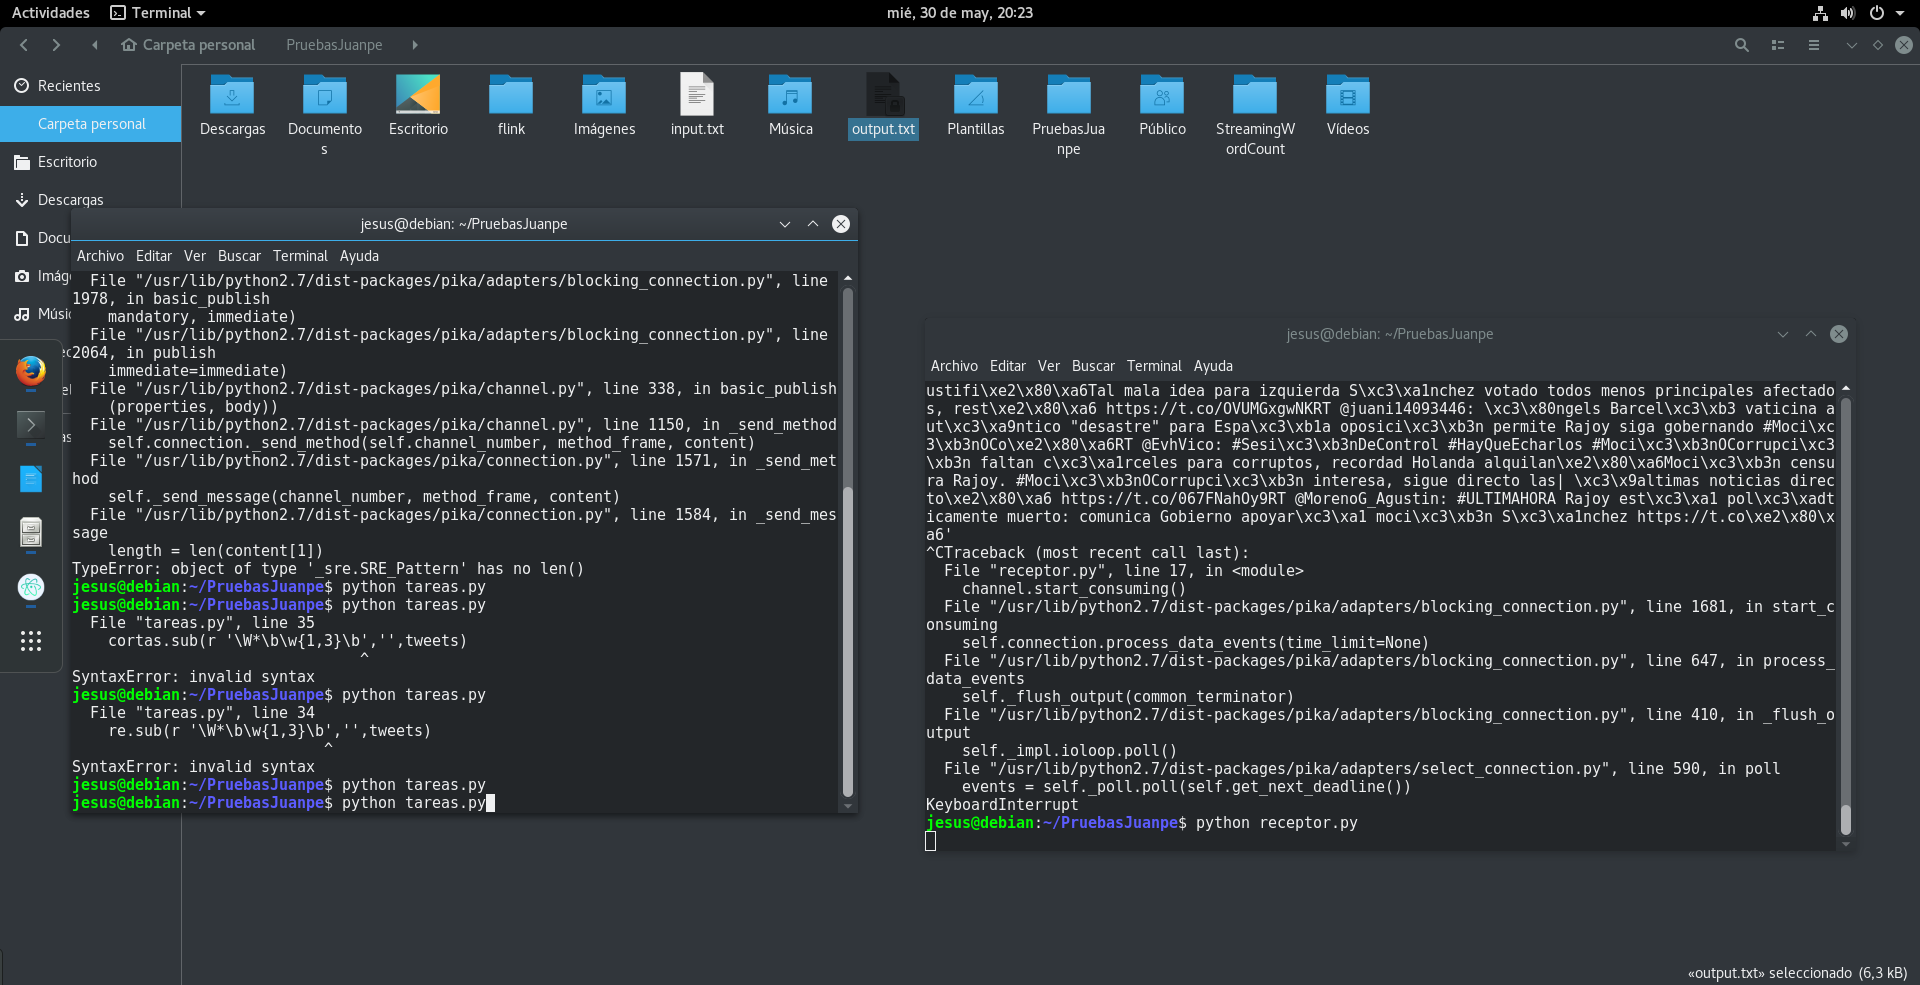
\includegraphics[scale=0.18]{16.png}
	\end{center}
\end{frame}

\begin{frame}{Palabras más publicadas en twitter}
\begin{center}
	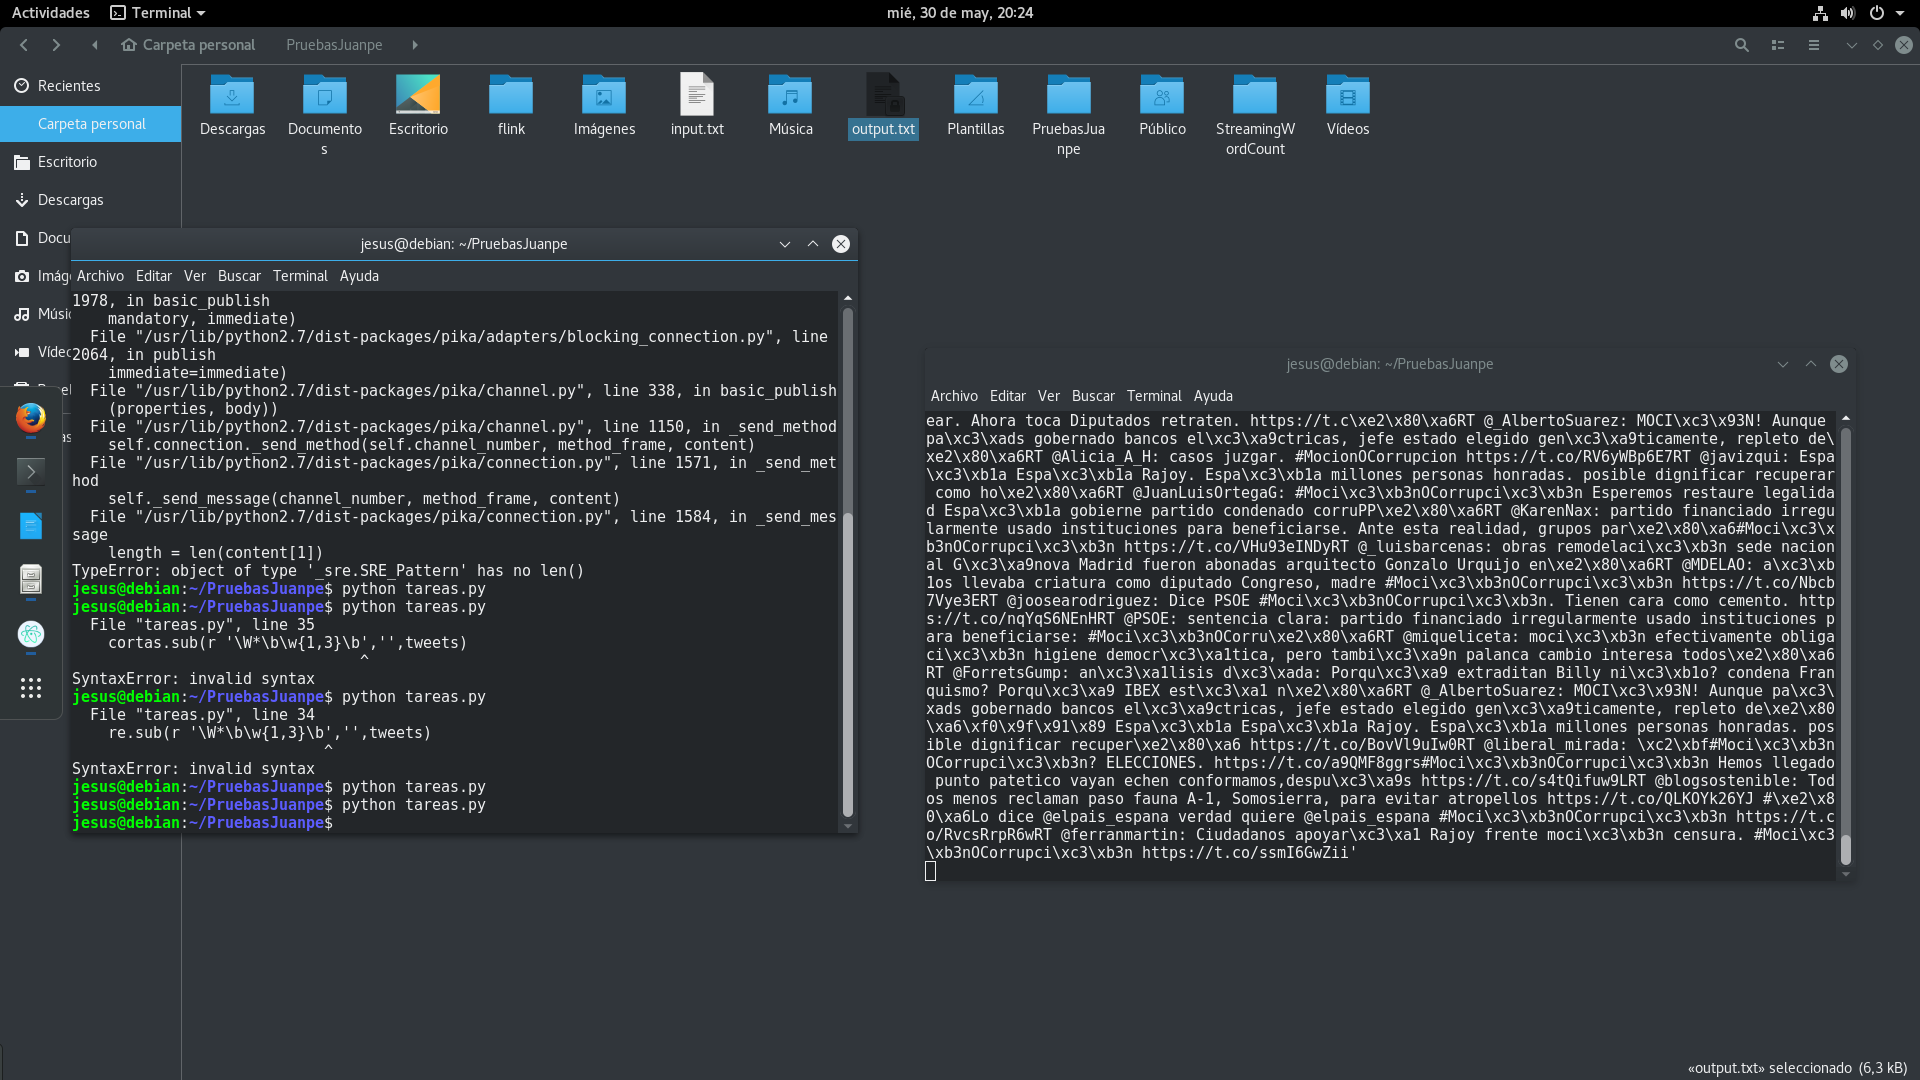
\includegraphics[scale=0.18]{17.png}
\end{center}
\end{frame}

\begin{frame}{Palabras más publicadas en twitter}
\begin{center}
	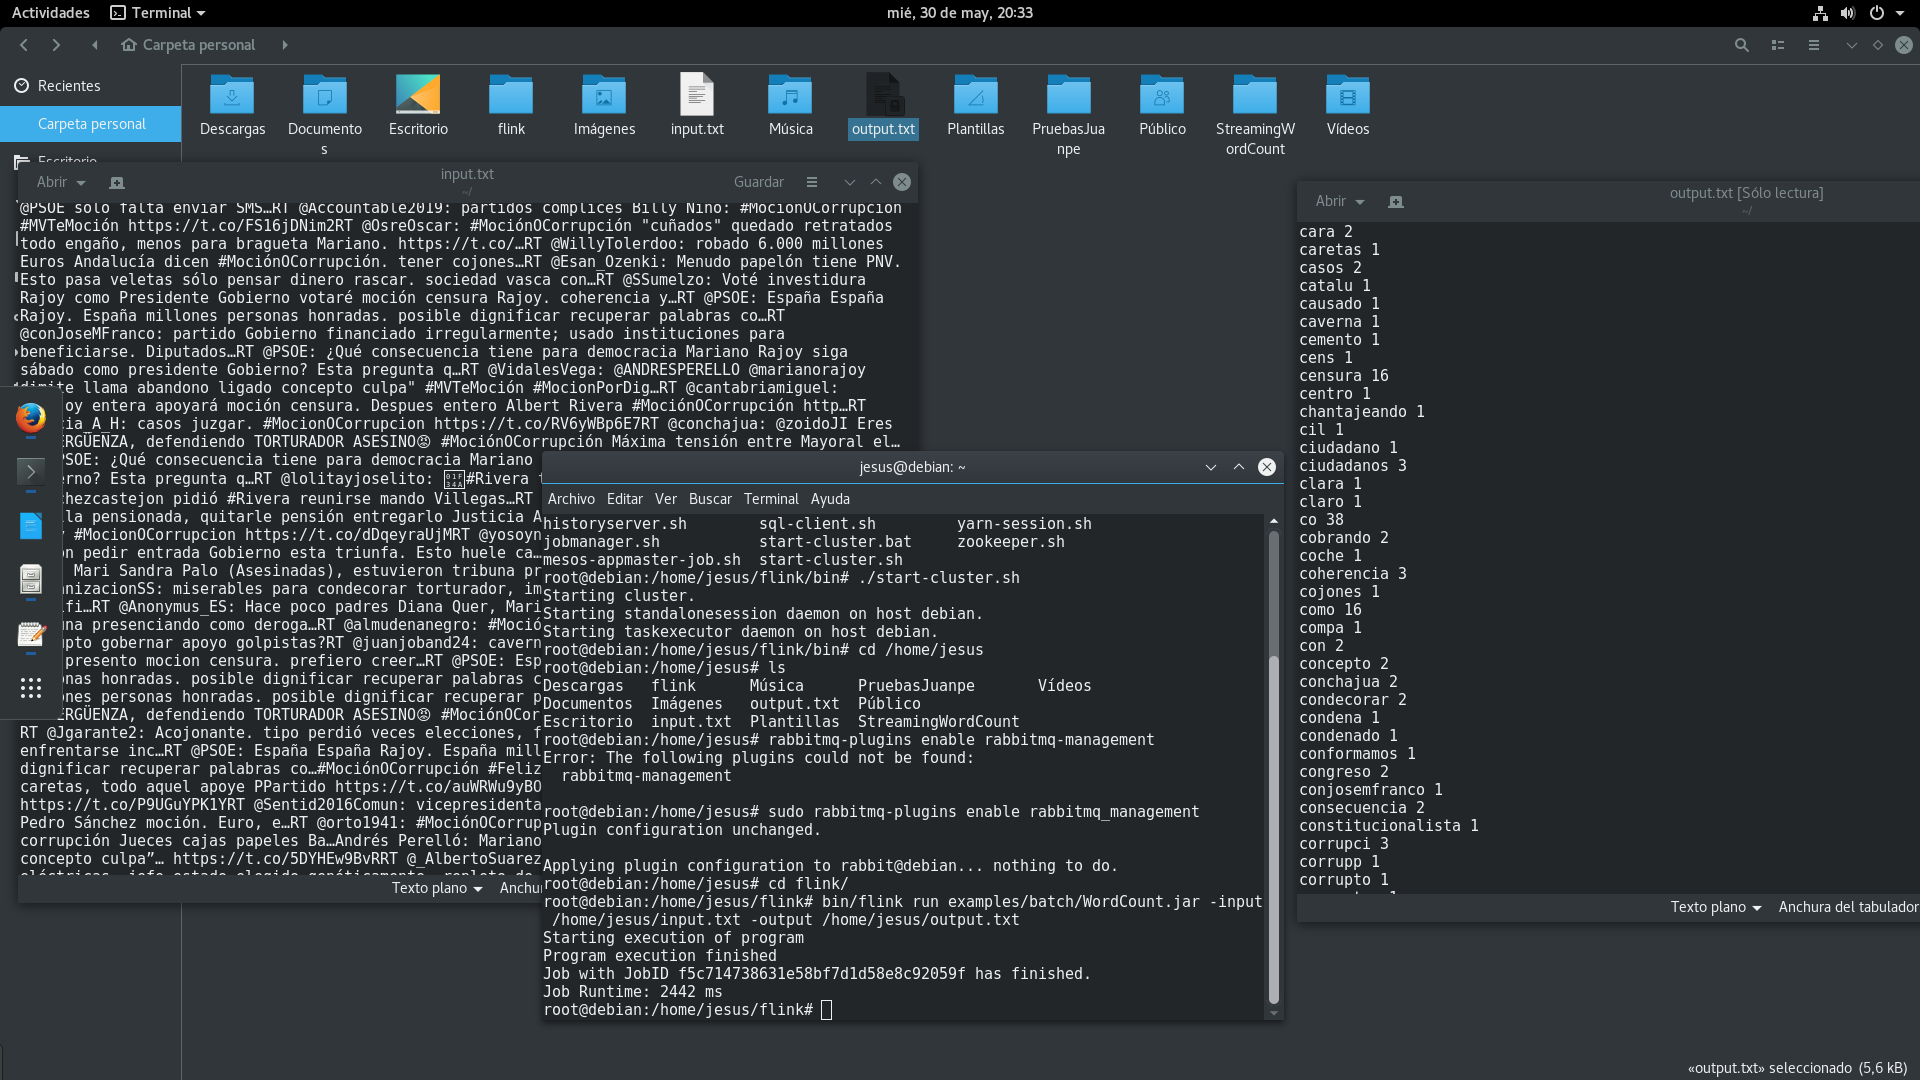
\includegraphics[scale=0.18]{18.png}
\end{center}
\end{frame}

\section{Problemas encontrados}
\begin{frame}{Problemas encontrados}
	\begin{block}{Problemas}
		\begin{itemize}
			\item No teníamos donde ejecutar Apache Flink.
			\item Apache Flink lanzaba multitud de excepciones.
		\end{itemize}
	\end{block}
\end{frame}

\section{Mejoras futuras}
\begin{frame}{Mejoras futuras}
\begin{block}{Mejoras}
	\begin{itemize}
		\item Mejorar la implementación de las palabras cortas (determinantes y preposiciones).
		\item Utilizar ``jpype'' para llamar a las clases Java desde Python, lo que nos ahorraría bastante trabajo.
	\end{itemize}
\end{block}
\end{frame}

\section{Referencias}
\begin{frame}{Referencias}
	\begin{itemize}
		\item \url{https://flink.apache.org/}
		\item \url{https://www.rabbitmq.com/}
		\item \url{https://en.wikipedia.org/wiki/Apache_Flink}
		\item \url{https://en.wikipedia.org/wiki/RabbitMQ}
		\item \url{https://www.adictosaltrabajo.com/tutoriales/introduccion-a-apache-flink/}
		\item \url{https://data-flair.training/blogs/install-configure-}\\\url{apache-flink-ubuntu/}
	\end{itemize}
\end{frame}


\end{document}


